
%%%%%%%%%%%%%%%%%%%%%%%%%%%%%%%%%%%%%%%%%
% Beamer Presentation
% LaTeX Template
% Version 1.0 (10/11/12)
%
% This template has been downloaded from:
% http://www.LaTeXTemplates.com
%
% License:
% CC BY-NC-SA 3.0 (http://creativecommons.org/licenses/by-nc-sa/3.0/)
%
%%%%%%%%%%%%%%%%%%%%%%%%%%%%%%%%%%%%%%%%%

%----------------------------------------------------------------------------------------
%	PACKAGES AND THEMES
%----------------------------------------------------------------------------------------

\documentclass{beamer}

\mode<presentation> {

	% The Beamer class comes with a number of default slide themes
	% which change the colors and layouts of slides. Below this is a list
	% of all the themes, uncomment each in turn to see what they look like.

	%\usetheme{default}
	%\usetheme{AnnArbor}
	%\usetheme{Antibes}
	%\usetheme{Bergen}
	%\usetheme{Berkeley}
	%\usetheme{Berlin}
	%\usetheme{Boadilla}
	%\usetheme{CambridgeUS}
	%\usetheme{Copenhagen}
	%\usetheme{Darmstadt}
	%\usetheme{Dresden}
	%\usetheme{Frankfurt}
	%\usetheme{Goettingen}
	%\usetheme{Hannover}
	%\usetheme{Ilmenau}
	%\usetheme{JuanLesPins}
	%\usetheme{Luebeck}
	%\usetheme{Madrid}
	%\usetheme{Malmoe}
	%\usetheme{Marburg}
	%\usetheme{Montpellier}
	%\usetheme{PaloAlto}
	\usetheme{Pittsburgh}
	%\usetheme{Rochester}
	%\usetheme{Singapore}
	%\usetheme{Szeged}
	%\usetheme{Warsaw}

	% As well as themes, the Beamer class has a number of color themes
	% for any slide theme. Uncomment each of these in turn to see how it
	% changes the colors of your current slide theme.

	%\usecolortheme{albatross}
	\usecolortheme{beaver}
	%\usecolortheme{beetle}
	%\usecolortheme{crane}
	%\usecolortheme{dolphin}
	%\usecolortheme{dove}
	%\usecolortheme{fly}
	%\usecolortheme{lily}
	%\usecolortheme{orchid}
	%\usecolortheme{rose}
	%\usecolortheme{seagull}
	%\usecolortheme{seahorse}
	%\usecolortheme{whale}
	%\usecolortheme{wolverine}

	%\setbeamertemplate{footline} % To remove the footer line in all slides uncomment this line
	%\setbeamertemplate{footline}[page number] % To replace the footer line in all slides with a simple slide count uncomment this line

	%\setbeamertemplate{navigation symbols}{} % To remove the navigation symbols from the bottom of all slides uncomment this line
}

\usepackage{graphicx} % Allows including images
\usepackage{booktabs} % Allows the use of \toprule, \midrule and \bottomrule in tables
%\usepackage{ctex}
\usepackage{multicol}
\usepackage{amsmath, bm}
\usepackage{fontspec}
\setsansfont{Calibri}[
    Path=Font/,
    Scale=0.9,
    Extension = .ttf,
    UprightFont=*-Regular,
    BoldFont=*-Bold,
    ItalicFont=*-Italic,
    BoldItalicFont=*-BoldItalic
    ]
\usepackage{unicode-math}
\setmathfont{Libertinus Math}% 使用默认的数学字体或你偏好的数学字体 Latin Modern Math/Libertinus Math

\usepackage{ragged2e}
\justifying\let\raggedright\justifying %两端对齐
\usepackage{tikz}
\usetikzlibrary{positioning}
\usetikzlibrary{calc}

\setbeamercolor{postit}{fg=black,bg=yellow!20} % 定义一个浅黄色背景
%----------------------------------------------------------------------------------------
%	TITLE PAGE
%----------------------------------------------------------------------------------------

\title[Asset Pricing]{\textbf{Asset Pricing}} % The short title appears at the bottom of every slide, the full title is only on the title page

\subtitle{5. Multi-Factors}

\author[Cheng Hang]{Cheng Hang} % Your name
\institute[DUFE] % Your institution as it will appear on the bottom of every slide, may be shorthand to save space
{School of Fintech \\
	Dongbei University of Finance \& Economics \\ % Your institution for the title page
	\medskip
	\textbf{chenghangch@qq.com}% Your email address
}
\date{\today} % Date, can be changed to a custom date



\AtBeginSection[]
{
	\begin{frame}{Content}
		\begin{columns}[t]
			\begin{column}{0.5\textwidth}
				\tableofcontents[sections={1-4},sectionstyle=show/shaded,subsectionstyle=show/shaded/hide]
			\end{column}
			\begin{column}{0.5\textwidth}
				\tableofcontents[sections={5-8},sectionstyle=show/shaded,subsectionstyle=show/shaded/hide]
			\end{column}
		\end{columns}
		\addtocounter{framenumber}{-1}
	\end{frame}
}

%----------------------------------------------
%	Begin
%----------------------------------------------

\begin{document}

\begin{frame}
	\titlepage % Print the title page as the first slide
\end{frame}
\section{The Fama-French Three-Factor Model}

% ---------------------------------------------------------
% 1. Introduction & Philosophy
% ---------------------------------------------------------
\begin{frame}{From CAPM to Multifactor Models}
	\begin{itemize}
		\item \textbf{The Context:} By the early 1990s, the empirical failure of CAPM was evident. Size and Book-to-Market (B/M) ratios predicted returns better than Beta.
		\item \textbf{The Seminal Work:} \href{https://www.sciencedirect.com/science/article/pii/0304405X93900235}{\textcolor{blue}{Fama and French (1993)}} proposed a three-factor model to capture these patterns.
		\item \textbf{The Core Philosophy:}\\
		\begin{beamercolorbox}[sep=0em,wd=\linewidth,rounded=true,shadow=true]{postit}
        \textit{``Size and Book-to-Market equity are not isolated anomalies, but proxies for non-diversifiable risks related to the underlying economic distress of firms.''}
    \end{beamercolorbox}
		\item \textbf{Theoretical Link:} In the language of \href{https://doi.org/10.2307/1913811}{\textcolor{blue}{Merton's ICAPM (1973)}}, SMB and HML mimic state variables that describe changes in the investment opportunity set.
	\end{itemize}
\end{frame}

% ---------------------------------------------------------
% 2. The Model Specification
% ---------------------------------------------------------
\begin{frame}{The Three-Factor Model Specification}
	The expected return of asset $i$ is given by:
	\begin{equation}
		E[R_{i}] - R_f = \beta_{i}(E[R_{M}] - R_{f}) + s_{i} E[SMB] + h_{i} E[HML]
	\end{equation}
	Where:
	\begin{itemize}
		\item $R_M - R_f$: The Market Risk Premium.
		\item \textbf{SMB} (Small Minus Big): The size factor premium.
		\item \textbf{HML} (High Minus Low): The value factor premium.
		\item $\beta_i, s_i, h_i$: The factor loadings (slopes) estimated via time-series regression.
	\end{itemize}
	
	\vspace{0.5cm}
	\footnotesize
	\textcolor{red}{Insight:} If the FF3 model holds, a portfolio constructed by mixing MKT, SMB, and HML lies on the Mean-Variance Frontier. The CAPM is a special case where $s_i = 0$ and $h_i = 0$.
\end{frame}

% ---------------------------------------------------------
% 3. Construction Details: The 2x3 Sort
% ---------------------------------------------------------
\begin{frame}{Factor Construction: The 2x3 Sort}
	To construct SMB and HML, Fama and French use a double sort to ensure the factors are relatively independent.
	
	\begin{itemize}
		\item \textbf{Universe:} All NYSE, AMEX, and NASDAQ stocks.
		\item \textbf{Sorting Variables:}
		\begin{enumerate}
			\item \textbf{Size (ME):} Market Equity at the end of June of year $t$.
			\item \textbf{Value (B/M):} Book Equity (BE) for the fiscal year ending in $t-1$ divided by Market Equity (ME) at the end of December $t-1$.
		\end{enumerate}
		\item \textbf{Breakpoints (Crucial Detail):}
		\begin{itemize}
			\item \textbf{Size:} NYSE Median (Splits into Small vs. Big).
			\item \textbf{B/M:} NYSE 30th and 70th percentiles (Splits into Low, Neutral, High).
		\end{itemize}
	\end{itemize}
	\textit{Note: Using NYSE breakpoints prevents the ``Small" portfolio from being dominated by thousands of tiny NASDAQ stocks.}
\end{frame}

% ---------------------------------------------------------
% 4. Construction Details: Timing
% ---------------------------------------------------------
\begin{frame}{Factor Construction: Timing and Lag}
	\textbf{Why the lag?}
	\begin{itemize}
		\item We match returns from \textbf{July of year $t$} to \textbf{June of year $t+1$} with accounting data from fiscal year ending in \textbf{$t-1$}.
		\item \textbf{Reason:} To avoid \textit{Look-Ahead Bias}.
		\item Most firms file their annual reports (10-K) months after the fiscal year-end. By waiting until July, we ensure the Book Equity data was actually known to investors at the time of portfolio formation.
	\end{itemize}
	
	\begin{table}[h]
		\centering
		\caption{The Six Portfolios (Value-Weighted)}
		\begin{tabular}{c|ccc}
			\hline
			& Low B/M (Growth) & Medium B/M & High B/M (Value) \\
			\hline
			Small & S/L & S/M & S/H \\
			Big   & B/L & B/M & B/H \\
			\hline
		\end{tabular}
	\end{table}
\end{frame}

% ---------------------------------------------------------
% 5. Factor Definitions
% ---------------------------------------------------------
\begin{frame}{Calculating SMB and HML}
	Based on the value-weighted returns of the six portfolios\\ ($S/L, S/M, S/H, B/L, B/M, B/H$):
	
	\begin{block}{SMB (Small Minus Big)}
		Measures the size effect, controlling for value:
		$$ SMB = \frac{1}{3}(S/L + S/M + S/H) - \frac{1}{3}(B/L + B/M + B/H) $$
	\end{block}
	
	\begin{block}{HML (High Minus Low)}
		Measures the value effect, controlling for size:
		$$ HML = \frac{1}{2}(S/H + B/H) - \frac{1}{2}(S/L + B/L) $$
	\end{block}
	
	\footnotesize
	See \href{https://mba.tuck.dartmouth.edu/pages/faculty/ken.french/data_library.html}{\textcolor{blue}{Kenneth French's Data Library}} for updated data.
\end{frame}

% ---------------------------------------------------------
% 6. Economic Mechanism
% ---------------------------------------------------------
\begin{frame}{Mechanism: Risk or Mispricing?}
	Why do SMB and HML earn positive premiums? This is the great debate of the 1990s.
	\vspace{5pt}
	\begin{columns}
		\column{0.5\textwidth}
		\textbf{1. The Rational View (Risk)} \\
		\href{https://doi.org/10.1111/j.1540-6261.1996.tb05202.x}{\textcolor{blue}{Fama and French (1996)}}
		\begin{itemize}
			\item \textbf{HML:} Proxies for \textit{financial distress}. Value firms are often fallen angels with high leverage and uncertain future earnings.
			\item \textbf{SMB:} Small firms are more sensitive to credit conditions and liquidity shocks.
		\end{itemize}
		
		\column{0.5\textwidth}
		\textbf{2. The Behavioral View (Mispricing)} \\
		\href{10.1111/j.1540-6261.1994.tb04772.x}{\textcolor{blue}{Lakonishok, Shleifer, Vishny (1994)}}
		\begin{itemize}
			\item Investors \textit{overreact} to past news.
			\item They drive prices of ``Growth" stocks too high and ``Value" stocks too low.
			\item HML return is the subsequent correction of these errors.
		\end{itemize}
	\end{columns}
\end{frame}

% ---------------------------------------------------------
% 7. Empirical Evidence: China
% ---------------------------------------------------------
\begin{frame}{Empirical Evidence in China: The Shell Value}
	Applying FF3 to China requires modification due to the unique institutional background.
	
	\begin{itemize}
		\item \href{https://doi.org/10.1016/j.jfineco.2019.03.008}{\textcolor{blue}{Liu, Stambaugh, and Yuan (2019)}}: \textbf{Size and Value in China}.
		\item \textbf{The Shell Value Problem:} In China, IPOs are tightly regulated. Failed firms are valuable as ``shells" for reverse mergers.
		\item \textbf{Consequence:} The smallest stocks (junk) often have high prices (low returns), contradicting the standard size effect.
		\item \textbf{Solution:} Exclude the bottom 30\% of stocks (Shells) when constructing factors.
		\item \textbf{Value Factor:} They find Earnings-to-Price (EP) works better than Book-to-Market (BM) in China.
	\end{itemize}
\end{frame}

\begin{frame}{Performance of CH-3 Model}
	\begin{table}
		\caption{Summary statistics for the CH-3 factors (Liu et al., 2019)}
		\small
		\begin{tabular}{lcccccc}
			\hline & & & & \multicolumn{3}{c} { Correlations } \\
			\cline { 5 - 7 } Factor & Mean & Std. dev. & $t$ -stat. & MKT & SMB & VMG \\
			\hline 
			MKT & $0.66$ & $8.09$ & $1.16$ & $1.00$ & $0.12$ & $-0.27$ \\
			SMB & $1.03$ & $4.52$ & $3.25$ & $0.12$ & $1.00$ & $-0.62$ \\
			VMG & $1.14$ & $3.75$ & $4.34$ & $-0.27$ & $-0.62$ & $1.00$ \\
			\hline
		\end{tabular}
	\end{table}
	\footnotesize
	\textit{Note: The CH-3 model (MKT, SMB, VMG) successfully explains most anomalies in China, except for high turnover and volatility.}
\end{frame}

% ---------------------------------------------------------
% 8. Methodology: Time Series
% ---------------------------------------------------------
\begin{frame}{Methodology 1: Time-Series Regression}
	How do we test if the model works?
	
	\begin{itemize}
		\item \textbf{Applicability:} Used when factors are \textbf{tradable portfolios} (like MKT, SMB, HML).
		\item \textbf{Procedure:} Run OLS for each test asset $i$ (e.g., 25 Size-B/M portfolios):
		$$ R_{it} - R_{ft} = \alpha_i + \beta_i MKT_t + s_i SMB_t + h_i HML_t + \varepsilon_{it} $$
		\item \textbf{The Test:}
		\begin{itemize}
			\item If the model is perfect, all intercepts $\alpha_i$ should be jointly zero.
			\item We use the \textbf{GRS Test} \href{Gibbons, Ross, and Shanken, 1989)}{\textcolor{blue}{(Gibbons, Ross, and Shanken, 1989)}} to test the null hypothesis: $\alpha_1 = \alpha_2 = ... = \alpha_N = 0$.
		\end{itemize}
		\item \textbf{Result:} FF3 significantly reduces $\alpha$ compared to CAPM, raising $R^2$ from $\sim 0.70$ to $>0.90$.
	\end{itemize}
\end{frame}

% ---------------------------------------------------------
% 9. Methodology: Fama-MacBeth
% ---------------------------------------------------------
\begin{frame}{Methodology 2: Fama-MacBeth Regression}
	Used when factors are non-tradable or to test if a characteristic predicts returns cross-sectionally.
	
	\begin{enumerate}
		\item \textbf{Step 1 (Time-Series):} Estimate factor betas ($\beta_{i,SMB}, \beta_{i,HML}$) for each asset using historical data.
		$$ R_{it} = a_i + \beta_i f_t + \epsilon_{it} $$
		\item \textbf{Step 2 (Cross-Section):} At each month $t$, run a cross-sectional regression of returns on the estimated betas:
		$$ R_{it} = \lambda_{0t} + \lambda_{t} \hat{\beta}_{i} + \alpha_{it} $$
		\item \textbf{Step 3 (Averaging):} The final estimate of the risk premium $\lambda$ is the time-series average of $\lambda_t$.
		$$ \hat{\lambda} = \frac{1}{T} \sum_{t=1}^{T} \lambda_t $$
	\end{enumerate}
	\textit{Advantage: Corrects for cross-sectional correlation in residuals.}
\end{frame}

% ---------------------------------------------------------
% 10. Limitations & Conclusion
% ---------------------------------------------------------
\begin{frame}{Limitations and Extensions}
	While FF3 was a paradigm shift, it is not the final theory.
	
	\begin{itemize}
		\item \textbf{Momentum:} FF3 cannot explain the momentum effect. Winners continue to win, but they don't necessarily have high SMB or HML loadings.
		\item \textbf{Profitability \& Investment:} FF3 ignores the ``Quality" dimension.
		\item \textbf{The Evolution:}
		\begin{itemize}
			\item $\rightarrow$ \textbf{Carhart (1997) 4-Factor Model}: Adds Momentum (MOM).
			\item $\rightarrow$ \textbf{Fama-French (2015) 5-Factor Model}: Adds Profitability (RMW) and Investment (CMA).
			\item $\rightarrow$ \textbf{q-Factor Model} (Hou, Xue, Zhang, 2015): Based on investment theory.
		\end{itemize}
	\end{itemize}
\end{frame}


\section{Fama and French fails again}

\subsection{Momentum}

\begin{frame}{The Challenge: Momentum}
	\begin{itemize}
		\item By the mid-1990s, the Fama-French Three-Factor Model (FF3) seemed to have conquered the asset pricing world, explaining Size and Value perfectly.
		\item However, one anomaly stood stubborn: \textbf{Momentum}.
		\item \href{https://doi.org/10.1111/j.1540-6261.1997.tb03808.x}{\textcolor{blue}{Carhart (1997)}}, a student of Fama, demonstrated that FF3 fails miserably to explain the returns of portfolios sorted by past performance.
	\end{itemize}
	
	\vspace{0.3cm}
	\begin{block}{Fama's Concession}
		Eugene Fama, the father of the Efficient Market Hypothesis, famously admitted:
		\begin{center}
			\textit{``The premier anomaly is momentum.''}
		\end{center}
		\footnotesize (\href{https://doi.org/10.1111/j.1540-6261.2008.01371.x}{\textcolor{blue}{Fama and French, 2008}}, \textit{Dissecting Anomalies})
	\end{block}
\end{frame}

% ---------------------------------------------------------
% 2. Construction Details (J&T 1993)
% ---------------------------------------------------------
\begin{frame}{Constructing Momentum: Jegadeesh and Titman (1993)}
	\begin{itemize}
		\item \textbf{Seminal Work:} \href{https://doi.org/10.1111/j.1540-6261.1993.tb04702.x}{\textcolor{blue}{Jegadeesh and Titman (1993)}} documented that strategies which buy past winners and sell past losers generate significant positive returns.
		\item \textbf{The Strategy $(J, K)$:}
		\begin{enumerate}
			\item \textbf{Formation Period ($J$):} Rank stocks based on their cumulative returns over the past $J$ months (usually $J=6$ or $12$).
			\item \textbf{Holding Period ($K$):} Hold the top decile (Winners) and short the bottom decile (Losers) for $K$ months.
			\item \textbf{The Skip-Month:} Standard practice skips the most recent month ($t-1$) to avoid \textit{short-term reversal} caused by microstructure noise (bid-ask bounce).
		\end{enumerate}
		\item \textbf{Standard Definition (MOM):} The "12-1" momentum uses returns from month $t-13$ to $t-2$.
	\end{itemize}
\end{frame}

% ---------------------------------------------------------
% 3. Why FF3 Fails (The Mechanism)
% ---------------------------------------------------------
\begin{frame}{Why is Momentum "Embarrassing" for FF3?}
	\begin{itemize}
		\item Intuitively, one might think FF3 could explain momentum. It cannot. In fact, FF3 makes the puzzle \textbf{worse}.
		\item \textbf{The Logic of Failure:}
		\begin{itemize}
			\item \textbf{Winners} (high past returns) tend to have high prices relative to book value $\rightarrow$ Low B/M $\rightarrow$ \textbf{Growth Stocks}.
			\item \textbf{Losers} (low past returns) tend to have low prices $\rightarrow$ High B/M $\rightarrow$ \textbf{Value Stocks}.
		\end{itemize}
		\item \textbf{FF3 Prediction:} Since Winners are "Growth" and Losers are "Value", FF3 predicts that Losers should earn \textit{higher} returns than Winners (due to the HML premium).
		\item \textbf{Reality:} Winners massively outperform Losers.
		\item \textbf{Result:} The FF3 $\alpha$ for a momentum strategy is often \textit{larger} than its raw return.
	\end{itemize}
\end{frame}

% ---------------------------------------------------------
% 4. The Carhart (1997) Four-Factor Model
% ---------------------------------------------------------
\begin{frame}{The Solution: Carhart (1997) Four-Factor Model}
	To resolve this, Mark Carhart simply added a momentum factor to the FF3 model. This became the standard for mutual fund performance evaluation.
	
	\begin{equation}
		R_{it} - R_{ft} = \alpha_i + \beta_i MKT_t + s_i SMB_t + h_i HML_t + \textcolor{red}{w_i UMD_t} + \varepsilon_{it}
	\end{equation}
	
	\begin{itemize}
		\item \textbf{UMD (Up Minus Down):} The return difference between the highest performing stocks (top 30\%) and the lowest performing stocks (bottom 30\%).
		\item \textbf{Interpretation:}
		\begin{itemize}
			\item If a mutual fund manager claims to have ``skill" ($\alpha > 0$), we check if they are just chasing momentum.
			\item If adding $UMD$ reduces $\alpha$ to zero, the manager has no skill, just a known style.
		\end{itemize}
	\end{itemize}
\end{frame}

% ---------------------------------------------------------
% 5. Explanations: Behavioral vs. Risk
% ---------------------------------------------------------
\begin{frame}{Explaining Momentum: Behavioral Finance}
	Since it is hard to argue that ``past high returns" represent a fundamental risk factor, Momentum fueled the rise of \textbf{Behavioral Finance}.
	
	\begin{itemize}
		\item \textbf{Underreaction \& Overreaction:}
		\begin{itemize}
			\item \href{https://doi.org/10.1016/S0304-405X(98)00027-0}{\textcolor{blue}{Barberis, Shleifer, and Vishny (1998)}}: Investors suffer from \textit{conservatism bias} (underreact to earnings news) and \textit{representativeness heuristic} (overreact to consistent patterns).
		\end{itemize}
		\item \textbf{Self-Attribution Bias:}
		\begin{itemize}
			\item \href{https://doi.org/10.1111/0022-1082.00077}{\textcolor{blue}{Daniel, Hirshleifer, and Subrahmanyam (1998)}}: Investors attribute success to skill and failure to bad luck, leading to continued overpricing of winners.
		\end{itemize}
		\item \textbf{Gradual Information Diffusion:}
		\begin{itemize}
			\item \href{https://doi.org/10.1111/0022-1082.00184}{\textcolor{blue}{Hong and Stein (1999)}}: Information travels slowly across heterogeneous investors.
		\end{itemize}
	\end{itemize}
\end{frame}

% ---------------------------------------------------------
% 6. Robustness (Global Evidence)
% ---------------------------------------------------------
\begin{frame}{Momentum is Everywhere}
	Is Momentum just a US data mining result? No.
	
	\begin{itemize}
		\item \href{https://doi.org/10.1111/jofi.12021}{\textcolor{blue}{Asness, Moskowitz, and Pedersen (2013), \textit{Value and Momentum Everywhere}}} found consistent momentum premiums across:
		\begin{itemize}
			\item \textbf{Markets:} US, UK, Europe, Japan.
			\item \textbf{Asset Classes:} Stocks, Bonds, Currencies, Commodities.
		\end{itemize}
		\item \textbf{The ``Twin" of Value:} They document a strong negative correlation between Value and Momentum strategies, suggesting they capture complementary risks or behavioral biases.
	\end{itemize}
\end{frame}


\begin{frame}{Momentum}
	\begin{figure}
		\centering
		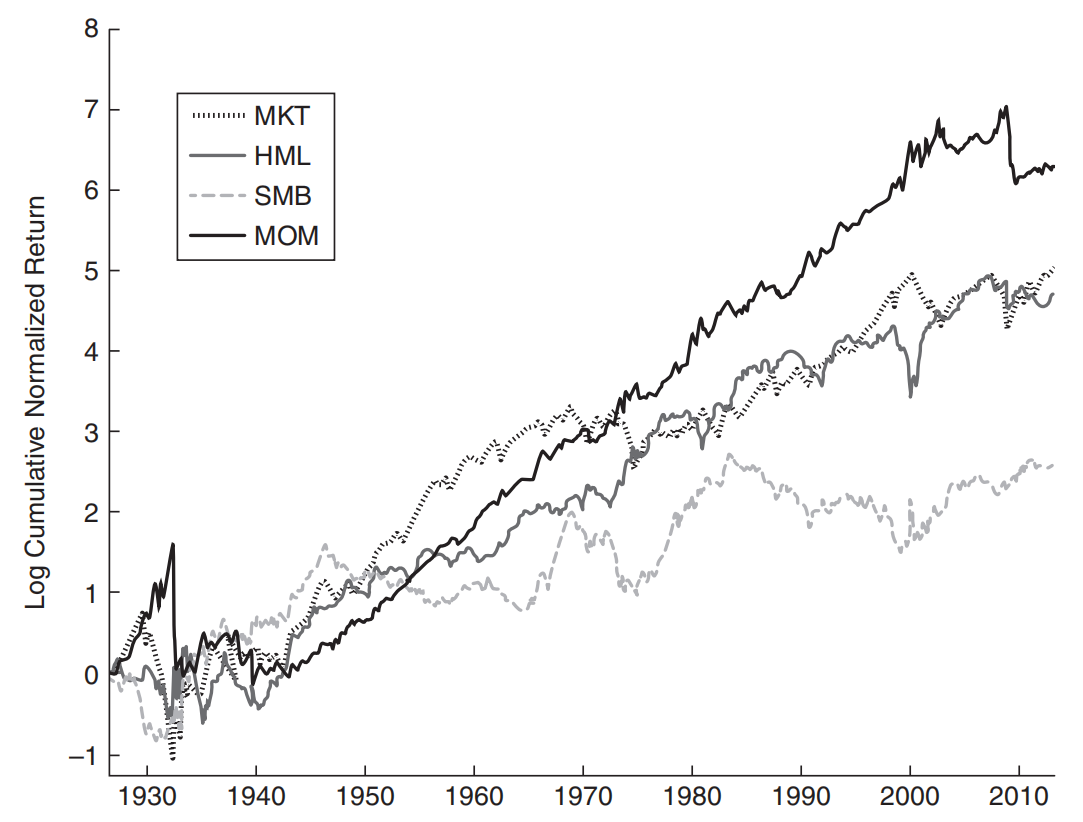
\includegraphics[width=0.7\linewidth]{Files/mom.png}
		\caption{Fama-French-Carhart Log Cumulative Normalized Factor Returns, 1926–2013}
		\label{fig:mom}
	\end{figure}
\end{frame}

% ---------------------------------------------------------
% Frame 1: The Setting - A vs B Shares
% ---------------------------------------------------------
\begin{frame}{Momentum in China: The A-share vs. B-share Puzzle}
	\begin{itemize}
		\item \textbf{The Puzzle:} While momentum is a robust global phenomenon, it is notably absent in China's A-share market (\href{https://doi.org/10.1111/j.1540-6261.2009.01532.x}{\textcolor{blue}{Chui, Titman, and Wei, 2010}}).
		\item \textbf{A Natural Experiment:} \href{https://doi.org/10.1093/rof/rfac010}{\textcolor{blue}{Chui, Subrahmanyam, and Titman (2022)}} exploit the unique dual-class structure in China to isolate the effect of investor clientele:
		\begin{itemize}
			\item \textbf{A-shares:} Dominated by domestic retail investors (often characterized as ``noise traders'').
			\item \textbf{B-shares:} Dominated by foreign institutional investors (more sophisticated).
			\item \textit{Crucial Point:} Both shares represent claims on the \textbf{same} underlying cash flows and voting rights.
		\end{itemize}
		\item \textbf{The Hypothesis:}
		\begin{enumerate}
			\item \textbf{A-shares (Noise):} High retail participation creates excessive noise trading. Market makers demand an inventory risk premium, leading to \textbf{Short-term Reversals}.
			\item \textbf{B-shares (Informed):} Institutions tend to underreact to fundamental signals (due to conservatism), leading to \textbf{Momentum}.
		\end{enumerate}
	\end{itemize}
\end{frame}

% ---------------------------------------------------------
% Frame 2: Empirical Findings & Mechanism
% ---------------------------------------------------------
\begin{frame}{Empirical Evidence: Clientele Matters}
	\begin{itemize}
		\item \textbf{Key Findings from Chui et al. (2022):}
		\begin{table}[h]
			\centering
			\small
			\begin{tabular}{lcc}
				\hline
				\textbf{Strategy} & \textbf{A-Shares} & \textbf{B-Shares} \\
				\hline
				\textbf{Momentum} (6-month) & Insignificant & \textbf{Significant} ($\sim$1.15\%/mo) \\
				\textbf{Reversal} (Monthly) & \textbf{Significant} & Insignificant \\
				\hline
			\end{tabular}
		\end{table}
		
		\item \textbf{Mechanism Analysis:}
		\begin{itemize}
			\item \textbf{A-shares:} The strong reversal effect (driven by liquidity provision to noise traders) effectively ``kills'' any potential momentum. Volatility is significantly higher in A-shares.
			\item \textbf{B-shares:} Momentum is stronger in B-shares with \textit{higher} institutional ownership, consistent with the theory that momentum arises from the underreaction of sophisticated investors to information.
		\end{itemize}
		
		\begin{block}{Conclusion}
			Momentum is not an inherent property of the asset's cash flows. Instead, it depends on the \textbf{investor clientele}. When noise traders dominate (A-shares), we see reversals; when sophisticated investors dominate (B-shares), we see momentum.
		\end{block}
	\end{itemize}
\end{frame}

% \subsection{Betting Against Beta}
% \begin{frame}{Betting Against Beta: Theoretical Background}
%     \textbf{The Security Market Line Puzzle:}
%     \begin{itemize}
%         \item Classic CAPM predicts a linear relation between beta and expected returns
%         \item Empirical evidence: The security market line is too flat (\textcolor{blue}{\href{https://doi.org/10.1111/j.1540-6261.1972.tb00971.x}{Black, Jensen, and Scholes, 1972}}; \textcolor{blue}{\href{https://doi.org/10.1111/j.1540-6261.1992.tb04398.x}{Fama and French, 1992}})
%         \item Low-beta stocks earn higher risk-adjusted returns than high-beta stocks
%     \end{itemize}

%     \textbf{Leverage and Margin Constraints:}
%     \begin{itemize}
%         \item Many investors face constraints on leverage (mutual funds, pension funds)
%         \item Constrained investors seeking high returns overweight high-beta assets
%         \item This demand pressure lowers expected returns of high-beta stocks
%         \item Creates arbitrage opportunity for unconstrained investors
%     \end{itemize}
% \end{frame}

% \begin{frame}{Betting Against Beta}
%     \textcolor{blue}{\href{https://doi.org/10.1016/j.jfineco.2013.10.005}{Frazzini and Pedersen (2014)}} introduces a model incorporating leverage and margin constraints that vary across investors and time. Their model predicts that constrained investors bid up high-beta assets, leading to low alpha for these assets. They provide a robust framework for understanding how funding constraints and liquidity risk influence asset pricing and investor behavior.
%     \begin{equation}
% R_{t+1}^{B A B}=\frac{1}{\beta_L} R_{L, t+1}^e-\frac{1}{\beta_H} R_{H, t+1}^e
% \end{equation}
% where $R_{L, t+1}^e$ is the excess return on the low-beta portfolio and
% $R_{H, t+1}^e$ the excess return on the high-beta portfolio.
% \end{frame}


% \begin{frame}{BAB Factor Construction: Technical Details}
%     \textbf{Step 1: Beta Estimation (Section 3.1)}
%     \begin{itemize}
%         \item Estimate beta as $\hat{\beta}_i^{ts} = \hat{\rho} \hat{\sigma}_i / \hat{\sigma}_m$, separating volatility and correlation
%         \item Volatility: One-year rolling standard deviation of daily log returns
%         \item Correlation: Five-year rolling correlation using overlapping three-day log returns (to control for nonsynchronous trading)
%         \item Minimum requirements: 120 trading days for volatility, 750 trading days for correlation
%         \item Shrinkage: $\hat{\beta}_i = w \hat{\beta}_i^{TS} + (1-w) \hat{\beta}^{XS}$ with $w=0.6$ and $\hat{\beta}^{XS}=1$ (Vasicek, 1973)
%     \end{itemize}
% \end{frame}

% \begin{frame}{BAB Factor Construction: Portfolio Formation}
%     \textbf{Step 2: Ranking and Weighting (Section 3.2)}
%     \begin{itemize}
%         \item Rank all securities in ascending order by estimated beta
%         \item Split at median: Low-beta ($\beta < \text{median}$) and high-beta ($\beta > \text{median}$)
%         \item Within each portfolio, use \textit{rank weighting}: securities weighted by their beta ranks
%         \item Weight formulas: Let $z_i = \text{rank}(\beta_{it})$ and $\bar{z} = \mathbf{1}'_n z / n$
%         \begin{equation*}
%             w_H = k(z - \bar{z})^+, \quad w_L = k(z - \bar{z})^-, \quad k = 2/\mathbf{1}'_n|z - \bar{z}|
%         \end{equation*}
%         \item By construction: $\mathbf{1}'_n w_H = \mathbf{1}'_n w_L = 1$
%     \end{itemize}
% \end{frame}

% \begin{frame}{BAB Factor Construction: The Long-Short Strategy}
%     \textbf{Step 3: Scaling and Self-Financing Portfolio}
%     \begin{itemize}
%         \item Both portfolios are rescaled to have ex-ante beta of one:
%         \begin{equation*}
%             R_{t+1}^{BAB} = \frac{1}{\beta_t^L}(R_{L,t+1} - r_f) - \frac{1}{\beta_t^H}(R_{H,t+1} - r_f)
%         \end{equation*}
%         where $\beta_t^L = \beta'_t w_L$ and $\beta_t^H = \beta'_t w_H$
%         \item Self-financing: Difference between excess returns (not dollar-neutral in risky securities)
%         \item Market-neutral: Zero beta by construction (ex-ante)
%         \item Rebalancing: Monthly at calendar month-end
%     \end{itemize}

%     \textbf{Example: US Equities}
%     \begin{itemize}
%         \item Average long position: \$1.40 in low-beta stocks (financed by shorting \$1.40 risk-free)
%         \item Average short position: \$0.70 in high-beta stocks (with \$0.70 earning risk-free rate)
%     \end{itemize}
% \end{frame}

% \begin{frame}{Subsequent Research: Key Developments Post-2014}
%     \textbf{Major Research Directions:}
%     \begin{enumerate}
%         \item \textbf{Mechanism Testing}: What drives the BAB anomaly?
%         \begin{itemize}
%             \item Is it leverage constraints, lottery preferences, or correlation effects?
%         \end{itemize}
%         \item \textbf{Conditional Performance}: When does BAB work and when does it fail?
%         \begin{itemize}
%             \item Time-varying profitability and market conditions
%         \end{itemize}
%         \item \textbf{Implementation Challenges}: Is BAB truly exploitable?
%         \begin{itemize}
%             \item Transaction costs, volatility timing, and practical constraints
%         \end{itemize}
%         \item \textbf{Volatility Dynamics}: How does BAB interact with market volatility?
%         \begin{itemize}
%             \item The volatility puzzle of beta anomaly
%         \end{itemize}
%     \end{enumerate}
% \end{frame}

% \begin{frame}{Asness et al. (2020): Betting Against Correlation}
%     \textbf{Core Question:} 
%     \begin{itemize}
%         \item Is the low-risk effect driven by leverage constraints or other mechanisms?
%     \end{itemize}
    
%     \vspace{0.3cm}
%     \textbf{Key Innovation: Decomposing Risk}
%     \begin{itemize}
%         \item Total risk = Systematic risk (beta) + Idiosyncratic volatility
%         \item Market volatility = Individual volatility $\times$ Correlation with market
%         \item Construct "Betting Against Correlation" (BAC) factor:
%         \begin{itemize}
%             \item Long low-correlation stocks
%             \item Short high-correlation stocks
%             \item Control for volatility differences
%         \end{itemize}
%     \end{itemize}
    
%     \vspace{0.3cm}
%     \textbf{Main Findings:}
%     \begin{itemize}
%         \item BAC factor earns significant returns similar to BAB
%         \item Correlation risk, not just volatility, drives low-risk premiums
%         \item Results hold internationally across 24 developed markets
%         \item Challenges pure leverage constraint explanation
%     \end{itemize}
% \end{frame}

% \begin{frame}{Asness et al. (2020): Theoretical Implications}
%     \textbf{Three Competing Theories Tested:}
%     \begin{enumerate}
%         \item \textbf{Leverage Constraints:} Predicts BAB works but not necessarily BAC
%         \item \textbf{Lottery Preferences:} Investors overvalue high-volatility (lottery-like) stocks
%         \begin{itemize}
%             \item Predicts betting against volatility works, but correlation less relevant
%         \end{itemize}
%         \item \textbf{Benchmarking/Agency Costs:} Managers avoid low-correlation stocks
%         \begin{itemize}
%             \item Tracking error concerns make low-correlation stocks unattractive
%             \item Predicts both BAB and BAC work
%         \end{itemize}
%     \end{enumerate}
    
%     \vspace{0.3cm}
%     \textbf{Conclusion:}
%     \begin{itemize}
%         \item Evidence most consistent with \textit{benchmarking/agency explanation}
%         \item Leverage constraints alone cannot explain the full pattern
%         \item Correlation with benchmark matters independently of total risk
%         \item Low-beta premium partly reflects low-correlation premium
%     \end{itemize}
% \end{frame}

% \begin{frame}{Cederburg and O'Doherty (2016): Conditional Performance}
%     \textbf{Research Question:}
%     \begin{itemize}
%         \item Does BAB performance vary systematically with market conditions?
%         \item Is the anomaly always exploitable, or only in certain states?
%     \end{itemize}
    
%     \vspace{0.3cm}
%     \textbf{Methodology:}
%     \begin{itemize}
%         \item Examine BAB returns conditional on:
%         \begin{enumerate}
%             \item Aggregate market volatility (VIX)
%             \item Market returns (bull vs. bear markets)
%             \item Funding liquidity conditions (TED spread)
%             \item Economic uncertainty measures
%         \end{enumerate}
%         \item Sample: US equities 1926-2012
%     \end{itemize}
    
%     \vspace{0.3cm}
%     \textbf{Key Findings:}
%     \begin{itemize}
%         \item BAB profits are \textit{highly time-varying} and \textit{predictable}
%         \item Performs well in low-volatility, high-sentiment periods
%         \item \textcolor{red}{Negative or zero returns} during high-volatility, crisis periods
%         \item Economically significant timing strategies exist
%     \end{itemize}
% \end{frame}

% \begin{frame}{Cederburg and O'Doherty (2016): Main Results}
%     \textbf{Conditional Return Patterns:}
%     \begin{itemize}
%         \item \textbf{High VIX periods:} BAB alpha $\approx 0\%$ per month (insignificant)
%         \item \textbf{Low VIX periods:} BAB alpha $> 1\%$ per month (highly significant)
%         \item Similar patterns with TED spread and market downturns
%     \end{itemize}
    
%     \vspace{0.3cm}
%     \textbf{Risk-Based Interpretation:}
%     \begin{itemize}
%         \item BAB exposes investors to \textit{funding liquidity risk}
%         \item Losses occur when constraints become more binding (consistent with F-P theory)
%         \item Time-varying risk premium may explain average returns
%         \item Challenges view of BAB as "pure alpha" or persistent mispricing
%     \end{itemize}
    
%     \vspace{0.3cm}
%     \textbf{Implications:}
%     \begin{itemize}
%         \item BAB is \textit{not} a stable, unconditional arbitrage
%         \item Requires sophisticated timing or risk management
%         \item Transaction costs may eliminate profits for realistic investors
%         \item Questions practical exploitability of the anomaly
%     \end{itemize}
% \end{frame}

% \begin{frame}{Novy-Marx and Velikov (2022): Critical Examination}
%     \textbf{Central Thesis:} "Betting against betting against beta"
%     \begin{itemize}
%         \item Challenges the robustness and economic significance of BAB
%         \item Examines whether BAB survives realistic trading costs
%     \end{itemize}
    
%     \vspace{0.3cm}
%     \textbf{Key Critiques:}
%     \begin{enumerate}
%         \item \textbf{Transaction Costs:}
%         \begin{itemize}
%             \item BAB requires frequent rebalancing (monthly)
%             \item High leverage ratios magnify trading costs
%             \item After costs, BAB profitability largely disappears
%         \end{itemize}
%         \item \textbf{Short-Sale Constraints:}
%         \begin{itemize}
%             \item High-beta stocks are expensive to short
%             \item Short rebate rates reduce net returns
%             \item Limits practical implementation
%         \end{itemize}
%         \item \textbf{Specification Issues:}
%         \begin{itemize}
%             \item BAB performance sensitive to portfolio construction choices
%             \item Rank weighting vs. other schemes matters
%             \item Shrinkage parameter choice affects results
%         \end{itemize}
%     \end{enumerate}
% \end{frame}

% \begin{frame}{Novy-Marx and Velikov (2022): Empirical Findings}
%     \textbf{Transaction Cost Analysis:}
%     \begin{itemize}
%         \item Gross BAB return: $\approx 0.70\%$ per month (1926-2015)
%         \item Estimated transaction costs: $\approx 0.50-0.60\%$ per month
%         \item \textcolor{red}{Net return: Close to zero or negative}
%         \item Costs higher for small-cap stocks where BAB is strongest
%     \end{itemize}
    
%     \vspace{0.3cm}
%     \textbf{Robustness Tests:}
%     \begin{itemize}
%         \item BAB returns decline significantly in recent decades
%         \item Performance weaker in large, liquid stocks (where costs are lower)
%         \item Alternative beta estimation methods yield different results
%         \item Equal-weighted portfolios perform better than rank-weighted
%     \end{itemize}
    
%     \vspace{0.3cm}
%     \textbf{Conclusion:}
%     \begin{itemize}
%         \item BAB may not be economically exploitable after realistic costs
%         \item Challenges interpretation as persistent market inefficiency
%         \item More consistent with limits-to-arbitrage explanation
%         \item Questions practical relevance for institutional investors
%     \end{itemize}
% \end{frame}

% \begin{frame}{Barroso, Detzel, and Maio (2025): The Volatility Puzzle}
%     \textbf{The Puzzle:}
%     \begin{itemize}
%         \item BAB factor has \textit{positive} exposure to volatility risk
%         \item Yet BAB earns positive average returns
%         \item Contradicts standard risk-return tradeoff
%     \end{itemize}
    
%     \vspace{0.3cm}
%     \textbf{Key Findings:}
%     \begin{enumerate}
%         \item \textbf{Volatility Exposure:}
%         \begin{itemize}
%             \item BAB loads positively on volatility innovations
%             \item Returns decline when market volatility unexpectedly rises
%             \item Similar pattern across international markets
%         \end{itemize}
%         \item \textbf{Time-Varying Volatility Risk Premium:}
%         \begin{itemize}
%             \item Volatility risk carries \textit{negative} premium (investors hedge volatility)
%             \item BAB's positive volatility exposure should reduce, not increase, returns
%             \item Creates a "double puzzle" for the beta anomaly
%         \end{itemize}
%         \item \textbf{Resolution Attempt:}
%         \begin{itemize}
%             \item Propose state-dependent volatility risk pricing
%             \item BAB volatility exposure beneficial in some states, harmful in others
%             \item Partial reconciliation, but puzzle remains
%         \end{itemize}
%     \end{enumerate}
% \end{frame}

% \begin{frame}{Barroso et al. (2025): Theoretical Implications}
%     \textbf{Challenge to Existing Explanations:}
%     \begin{itemize}
%         \item \textbf{Leverage Constraints:} Cannot explain why high volatility exposure is rewarded
%         \item \textbf{Lottery Preferences:} Predicts negative correlation with volatility
%         \item \textbf{Benchmarking:} Silent on volatility dynamics
%     \end{itemize}
    
%     \vspace{0.3cm}
%     \textbf{New Perspective:}
%     \begin{itemize}
%         \item BAB returns may partly compensate for \textit{volatility timing risk}
%         \item Low-beta stocks have more stable returns (lower vol-of-vol)
%         \item High-beta stocks have time-varying risk that investors dislike
%         \item Suggests a "volatility stability premium" component
%     \end{itemize}
    
%     \vspace{0.3cm}
%     \textbf{Empirical Contributions:}
%     \begin{itemize}
%         \item Document systematic pattern across 30+ markets
%         \item Develop volatility-adjusted BAB strategies
%         \item Show puzzle persists even after controlling for other factors
%         \item Call for new theoretical models incorporating volatility dynamics
%     \end{itemize}
% \end{frame}

% \begin{frame}{Synthesis: Where Does the Literature Stand?}
%     \textbf{Areas of Consensus:}
%     \begin{itemize}
%         \item Low-beta stocks outperform high-beta stocks on risk-adjusted basis
%         \item Effect is pervasive across markets and time periods
%         \item Multiple mechanisms likely contribute (not a single explanation)
%     \end{itemize}
    
%     \vspace{0.3cm}
%     \textbf{Ongoing Debates:}
%     \begin{enumerate}
%         \item \textbf{Economic Exploitability:}
%         \begin{itemize}
%             \item Novy-Marx \& Velikov: Transaction costs eliminate profits
%             \item Others: BAB remains profitable for low-cost traders
%         \end{itemize}
%         \item \textbf{Risk vs. Mispricing:}
%         \begin{itemize}
%             \item Cederburg \& O'Doherty: Time-varying risk premium
%             \item Frazzini \& Pedersen: Persistent constraint-driven mispricing
%         \end{itemize}
%         \item \textbf{Driving Mechanism:}
%         \begin{itemize}
%             \item Asness et al.: Benchmarking and correlation matter
%             \item Barroso et al.: Volatility dynamics play a role
%             \item Original: Leverage constraints primary driver
%         \end{itemize}
%     \end{enumerate}
% \end{frame}

% \begin{frame}{Implications for Future Research}
%     \textbf{Open Questions:}
%     \begin{enumerate}
%         \item \textbf{Volatility Puzzle:} How to reconcile positive volatility exposure with positive returns?
%         \item \textbf{Declining Profitability:} Has anomaly weakened due to arbitrage capital?
%         \item \textbf{Optimal Implementation:} Best portfolio construction and rebalancing strategies?
%         \item \textbf{International Differences:} Why does BAB perform differently across countries?
%         \item \textbf{Factor Interaction:} How does BAB relate to quality, momentum, value factors?
%     \end{enumerate}
    
%     \vspace{0.3cm}
%     \textbf{Practical Implications:}
%     \begin{itemize}
%         \item BAB strategies require careful cost management
%         \item Timing and risk management are crucial
%         \item May work best as part of diversified factor portfolio
%         \item Need for continuous monitoring of market conditions
%     \end{itemize}
    
%     \vspace{0.3cm}
%     \textbf{Theoretical Needs:}
%     \begin{itemize}
%         \item Models incorporating volatility dynamics and time-varying constraints
%         \item Better understanding of investor heterogeneity and delegated portfolio management
%         \item Integration with behavioral finance theories
%     \end{itemize}
% \end{frame}


% \begin{frame}{Growth of the firm}
% 	\begin{itemize}
% 		\item Variables that capture \textbf{growth of a firm’s assets}, such as capital
% 		expenditures and total asset growth (\href{ https://doi.org/10.1017/S0022109000003173}{\textcolor{blue}{Titman, Wei, and Xie 2004}}, \href{https://doi.org/10.1111/j.1540-6261.2008.01370.x}{\textcolor{blue}{Cooper, Gulen, and Schill 2008}}), are negatively associated with subsequent returns.
% 		\item  The same is true for variables that capture growth of a firm’s liabilities, including measures of equity and debt issuance (\href{https://www.sciencedirect.com/science/article/pii/0304405X9400817K}{\textcolor{blue}{Spiess and Affleck-Graves 1995}, \href{https://www.sciencedirect.com/science/article/pii/S0304405X99000318}{\textcolor{blue}{1999}}}). Poor returns following initial public offerings (IPOs) may be a related phenomenon (\href{https://doi.org/10.1111/0022-1082.104624}{\textcolor{blue}{Carter, Dark, and Singh 1998}}, \href{https://onlinelibrary.wiley.com/doi/10.1111/1540-6261.00478}{\textcolor{blue}{Ritter and Welch 2002}}).
% 	\end{itemize}
% \end{frame}

% \begin{frame}{Profitability}
% 	\begin{itemize}
% 		\item \href{https://www.sciencedirect.com/science/article/pii/S0304405X13000044}{\textcolor{blue}{Novy-Marx (2013)}} shows that firms with higher ratios of gross \textbf{profitability} to book assets have higher subsequent returns. Gross profitability differs from current accounting earnings in that it adds back a number of corporate expenses that may enhance the long-run prospects of the firm, including advertising, sales commissions, and R\&D. Thus, while the accruals literature argues that the market gives firms too much credit for certain actions that do add to current earnings but are unproductive in the long run, the argument here is that the market gives insufficient credit for some actions that are productive in the long run but do not contribute to current earnings.
% 	\end{itemize}
% \end{frame}

\section{Why alpha still exists?}

\begin{frame}{Where Did the $\alpha$ Come From?}
    \textbf{The Fundamental Question in Anomaly Research:}
    \begin{itemize}
        \item After controlling for systematic risk factors, why do some portfolios earn excess returns?
        \item Is alpha real profit opportunity, compensation for risk, or statistical artifact?
    \end{itemize}
    
    \vspace{0.3cm}
    \textbf{Three Possible Explanations:}
    \begin{enumerate}
        \item \textbf{Model Misspecification} (Omitted variable problem)
        \begin{itemize}
            \item Missing risk factors that explain returns
            \item Alpha captures compensation for unmeasured systematic risk
        \end{itemize}
        \item \textbf{Statistical Luck} (Type I error and data mining)
        \begin{itemize}
            \item $\alpha$ not significantly different from zero
            \item Result of multiple testing or p-hacking
        \end{itemize}
        \item \textbf{Genuine Mispricing} (Market inefficiency)
        \begin{itemize}
            \item Behavioral biases or institutional frictions
            \item But why does mispricing persist?
        \end{itemize}
    \end{enumerate}
\end{frame}

\begin{frame}{Understanding Alpha: Formal Definition}
    \textbf{In a K-Factor Model:}
    \begin{equation*}
        R_{i,t} - r_{f,t} = \alpha_i + \sum_{k=1}^{K} \beta_{i,k} F_{k,t} + \varepsilon_{i,t}
    \end{equation*}
    
    \vspace{0.2cm}
    \textbf{Alpha Represents:}
    \begin{itemize}
        \item Expected return that cannot be explained by exposure to known risk factors
        \item Intercept in the time-series regression
        \item Average abnormal return per period
    \end{itemize}
    
    \vspace{0.3cm}
    \textbf{Economic Interpretation Is Model-Dependent:}
    \begin{itemize}
        \item \textbf{CAPM alpha:} Return unexplained by market risk
        \item \textbf{Fama-French 3-factor alpha:} Return beyond market, size, and value
        \item \textbf{Carhart 4-factor alpha:} Adding momentum
    \end{itemize}

    \textit{An anomaly's alpha is only meaningful relative to a specific asset pricing model}
\end{frame}

\begin{frame}[allowframebreaks]{Explanation 1: Omitted Risk Factors}
    \textbf{The Rational Asset Pricing View:}
    \begin{itemize}
        \item What appears as alpha may be compensation for risk we have not modeled
        \item \textcolor{blue}{\href{https://doi.org/10.1142/9789814417358_0001}{Ross (1976)}} Arbitrage Pricing Theory: Returns determined by multiple systematic risks
        \item \textcolor{blue}{\href{https://onlinelibrary.wiley.com/doi/10.1111/j.1540-6261.2011.01671.x}{Cochrane (2011)}}: "Discount rates" or "expected returns" reflect systematic risk
    \end{itemize}

    \textbf{Historical Pattern: Yesterday's Alpha Becomes Today's Beta}
    \begin{itemize}
        \item \textbf{1980s:} Size effect discovered $\rightarrow$ SMB factor (Banz, 1981)
        \item \textbf{1990s:} Value premium $\rightarrow$ HML factor (Fama and French, 1992)
        \item \textbf{1990s:} Momentum $\rightarrow$ UMD factor (Jegadeesh and Titman, 1993)
        \item \textbf{2010s:} Profitability and investment $\rightarrow$ RMW and CMA (Fama and French, 2015)
    \end{itemize}
    
    \vspace{1cm}
    \textbf{The Proliferation Problem:}
    \begin{itemize}
        \item \textcolor{blue}{\href{https://doi.org/10.1093/rfs/hhv059}{Harvey, Liu, and Zhu (2016)}}: 316 factors documented in top journals
        \item \textcolor{blue}{\href{https://doi.org/10.1093/rfs/hhy131}{Hou, Xue, and Zhang (2020)}}: Most anomalies fail to replicate
        \item Are these genuine risk factors or just data mining artifacts?
    \end{itemize}
\end{frame}

\begin{frame}{The Risk-Based Interpretation}
    \textbf{Arguments for Risk-Based Explanation:}
    
    \vspace{0.2cm}
    \textbf{1. Theoretical Foundation:}
    \begin{itemize}
        \item \textcolor{blue}{\href{https://doi.org/10.2307/1913811}{Merton (1973) ICAPM}}: Multiple state variables affect marginal utility
        \item \textcolor{blue}{\href{https://doi.org/10.1142/9789814417358_0001}{Ross (1976) APT}}: Multiple systematic risk sources
        \item Anomalies may capture these unmeasured state variables
    \end{itemize}
    
    \vspace{0.3cm}
    \textbf{2. Empirical Patterns Consistent with Risk:}
    \begin{itemize}
        \item \textbf{Time-varying returns:} Higher returns when risk aversion is high
        \item \textbf{Comovement:} Anomaly portfolios move together in bad times
        \item \textbf{Macroeconomic sensitivity:} Returns correlate with business cycles
    \end{itemize}
    
    \vspace{0.3cm}
    \textbf{3. Examples of Risk-Based Stories:}
    \begin{itemize}
        \item \textbf{Value premium:} Distress risk \href{https://doi.org/10.1111/j.1540-6261.1996.tb05202.x}{\textcolor{blue}{(Fama and French, 1996)}}
        \item \textbf{Size premium:} Greater exposure to economic downturns
        \item \textbf{Momentum:} Compensation for crash risk \href{https://doi.org/10.1016/j.jfineco.2015.12.002}{\textcolor{blue}{(Daniel and Moskowitz, 2016)}} 
        \item \textbf{Low volatility:} Funding liquidity risk \href{https://doi.org/10.1016/j.jfineco.2013.10.005}{\textcolor{blue}{(Frazzini and Pedersen, 2014)}} 
    \end{itemize}
\end{frame}

\begin{frame}[allowframebreaks]{Explanation 2: Data Mining and Multiple Testing}
    \textbf{The Statistical Problem:}
    \begin{itemize}
        \item With hundreds of potential predictors, some will appear significant by chance
        \item Traditional 5\% significance level: 1 in 20 ``discoveries" are false positives
        \item Publication bias: Only significant results get published (``file drawer problem")
    \end{itemize}
    
    \vspace{0.3cm}
    \textbf{Key Research on Multiple Testing:}
    \begin{itemize}
        \item \textcolor{blue}{\href{https://doi.org/10.1093/rfs/hhv059}{Harvey, Liu, and Zhu (2016)}}:
        \begin{itemize}
            \item Document 316 factors published in top journals
            \item Propose raising hurdle to t-stat $> 3.0$ (not 1.96) for new factors
            \item Bonferroni correction for multiple testing
        \end{itemize}
        \item \textcolor{blue}{\href{https://doi.org/10.1111/jofi.12365}{McLean and Pontiff (2016)}}:
        \begin{itemize}
            \item Anomaly returns decline by 26\% (equal-weighted) after publication
            \item 32\% decline for microcap stocks
            \item Evidence of both arbitrage and data mining
        \end{itemize}
    \end{itemize}

    \textbf{The Replication Crisis:}
    \begin{itemize}
        \item \textcolor{blue}{\href{https://doi.org/10.1093/rfs/hhaa018}{Chordia, Goyal, and Saretto (2020)}}: The proportion of false rejections under single hypothesis testing is about 45\%.
        \item \textcolor{blue}{\href{https://doi.org/10.1111/jofi.12951}{Harvey and Liu (2020)}}: This paper introduces a bootstrap-based framework to systematically evaluate the ``factor zoo," finding that most newly proposed factors provide no incremental explanatory power over existing common factors when properly correcting for multiple testing.
    \end{itemize}
\end{frame}

\begin{frame}{The Replication Crisis in Detail}
    \textbf{\href{https://doi.org/10.1093/rfs/hhy131}{\textcolor{blue}{Hou, Xue, and Zhang (2020)}}: ``Replicating Anomalies"}
    \begin{itemize}
        \item Attempt to replicate 452 anomalies from 447 studies
        \item Only 18\% are significant at 5\% level
        \item 85\% when focusing on microcaps (liquidity issues)
    \end{itemize}
    
    \vspace{0.3cm}
    \textbf{Reasons for Replication Failures:}
    \begin{enumerate}
        \item \textbf{Data errors:} Mistakes in original implementation
        \item \textbf{Specification choices:} 
        \begin{itemize}
            \item Different ways to measure variables
            \item Choice of breakpoints, weighting schemes
            \item Time periods and sample selection
        \end{itemize}
        \item \textbf{Microcap bias:}
        \begin{itemize}
            \item Many anomalies driven by smallest, illiquid stocks
            \item Not economically exploitable due to transaction costs
        \end{itemize}
        \item \textbf{Pure data mining:} Never real to begin with
    \end{enumerate}

    \textbf{Implication:} A significant fraction of published anomalies are likely false positives
\end{frame}

\begin{frame}{Beyond the U.S.: China and the New Anomaly Frontier}
    \begin{itemize}
        \item \textbf{China replication evidence:}
        \begin{itemize}
            \item \href{https://doi.org/10.1016/j.pacfin.2022.101739}{\textcolor{blue}{Han and Shi (2022)}}: among 62 Chinese anomalies, trading-friction effects are the strongest and sentiment is a major state variable.
            \item \href{https://doi.org/10.1287/mnsc.2023.4904}{\textcolor{blue}{Li, Liu, Liu, and Wei (2024)}}: 83.37\% of 469 anomaly variables fail under reliable A-share breakpoints and value-weighted tests.
            \item \href{https://eng.pbcsf.tsinghua.edu.cn/dfiles/wp6.pdf}{\textcolor{blue}{Hou, Qiao, and Zhang (August 2024)}}: only 38 of 454 Chinese raw strategies survive a multiple-testing hurdle, and none survive after risk adjustment.
        \end{itemize}
        \item \textbf{Recent frontier:}
        \begin{itemize}
            \item \href{https://doi.org/10.1093/rfs/hhad094}{\textcolor{blue}{Li, Shan, Tang, and Yao (2024)}} use earnings-call climate text to measure priced transition risk.
            \item \href{https://doi.org/10.1016/j.jfineco.2024.103952}{\textcolor{blue}{He, Su, and Yu (2024)}} show that subjective macro expectations time many classic anomalies.
            \item \href{https://doi.org/10.1093/rapstu/raaf001}{\textcolor{blue}{M\"uller and Schmickler (2025)}} show anomaly interactions are economically large and non-additive.
        \end{itemize}
    \end{itemize}

    \vspace{0.2cm}
    \textbf{Teaching point:} factor models should now be judged not only on U.S. size, value, and momentum, but also on \textbf{China portability}, \textbf{multiple-testing robustness}, and \textbf{new-information signals}.
\end{frame}

\begin{frame}{Explanation 3: Genuine Mispricing}
    \textbf{The Behavioral Finance View:}
    \begin{itemize}
        \item Investors are not fully rational
        \item Systematic biases lead to predictable mispricing
        \item Arbitrage is limited by frictions and risks
    \end{itemize}
    
    \vspace{0.3cm}
    \textbf{Key Behavioral Mechanisms:}
    \begin{enumerate}
        \item \textbf{Cognitive Biases:}
        \begin{itemize}
            \item Overconfidence, overreaction, underreaction
            \item \textcolor{blue}{\href{https://onlinelibrary.wiley.com/doi/abs/10.1111/j.1540-6261.1985.tb05004.x}{De Bondt and Thaler (1985)}}: Overreaction reversal
            \item \textcolor{blue}{\href{https://onlinelibrary.wiley.com/doi/10.1111/j.1540-6261.1993.tb04702.x}{Jegadeesh and Titman (1993)}}: Underreaction momentum
        \end{itemize}
        \item \textbf{Sentiment and Limits to Arbitrage:}
        \begin{itemize}
            \item \textcolor{blue}{\href{https://doi.org/10.1111/j.1540-6261.1997.tb03807.x}{Shleifer and Vishny (1997)}}: Limits to arbitrage
            \item \textcolor{blue}{\href{https://doi.org/10.1111/j.1540-6261.2006.00885.x}{Baker and Wurgler (2006)}}: Investor sentiment
        \end{itemize}
        \item \textbf{Institutional Frictions:}
        \begin{itemize}
            \item Short-sale constraints
            \item Agency problems and career concerns
            \item Benchmarking and tracking error constraints
        \end{itemize}
    \end{enumerate}
\end{frame}

\begin{frame}{Why Does Mispricing Persist?}
    \textbf{The Persistence Puzzle:}
    \begin{itemize}
        \item If anomalies represent mispricing, why doesn't arbitrage eliminate them?
        \item Many anomalies documented for decades, still present today
    \end{itemize}
    
    \vspace{0.3cm}
    \textbf{Limits to Arbitrage (Shleifer and Vishny, 1997):}
    \begin{enumerate}
        \item \textbf{Fundamental Risk:}
        \begin{itemize}
            \item Mispricing may worsen before correction
            \item Long horizons required, but capital is impatient
        \end{itemize}
        \item \textbf{Noise Trader Risk:}
        \begin{itemize}
            \item Sentiment can drive prices further from fundamentals
            \item Creates mark-to-market losses for arbitrageurs
        \end{itemize}
        \item \textbf{Implementation Costs:}
        \begin{itemize}
            \item Transaction costs, short-sale constraints
            \item \textcolor{blue}{\href{https://doi.org/10.1093/rfs/hhv063}{Novy-Marx and Velikov (2016)}}: Many anomalies unprofitable after costs
        \end{itemize}
        \item \textbf{Synchronization Risk:}
        \begin{itemize}
            \item Redemptions force liquidation at worst times
            \item Discourages contrarian strategies
        \end{itemize}
    \end{enumerate}
\end{frame}

\begin{frame}{But If the model is wrong? (When FF3 Fails)}
         \textbf{The ``Risk-Based" Fix (Save EMH)}
        \begin{itemize}
            \item \textit{Logic:} Alpha is just compensation for a \textbf{missing risk factor}.
            \item \textit{Action:} Augment the model (SDF Engineering).
            \item \textit{Evolution:} Carhart (4-factor) $\rightarrow$ Fama-French (5-factor) $\rightarrow$ q-factor (Hou, Xue, Zhang).
        \end{itemize}
\end{frame}

\end{document}
